\begin{frame}
	\frametitle{A Base de Sinais de Voz}
	\only<1>{
		\framesubtitle{Coleta dos dados}
		\begin{itemize}
			\item 20 pessoas.
			\item Ambos sexos.
			\item Idades entre 7 e 67 anos.
			\item Dígitos falados de 0 a 9.
			\item Língua portuguesa e inglesa.
			\item Total de 820 sinais entre genuínos e falsificados.
			\item Quantização de 16 bits.
			\item Taxa de amostragem 44100Hz.
		\end{itemize}
	}
	\only<2>{
		\framesubtitle{Organização dos dados}
		\begin{textblock*}{\linewidth}(0cm,0.4cm)
			\begin{figure}[t]
				\centering
				\subfloat[0.33\textwidth][Base em nível 1]{
					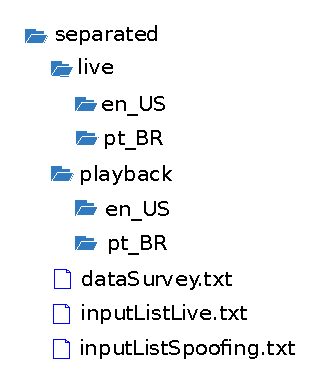
\includegraphics{../monography/images/directoryStructLevel01.pdf}
					\label{fig:directorystructlevel01}
				}
				\subfloat[0.33\textwidth][Base em nível 2]{
					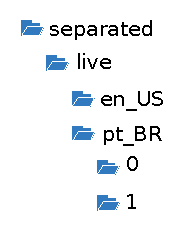
\includegraphics{../monography/images/directoryStructLevel02.pdf}
					\label{fig:directorystructlevel02}
				}
				\subfloat[0.33\textwidth][Base em nível 3]{
					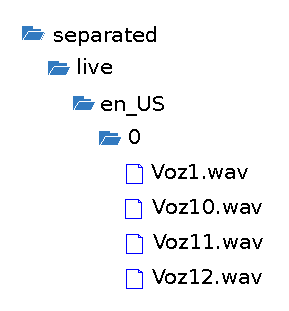
\includegraphics{../monography/images/directoryStructLevel03.pdf}
					\label{fig:directorystructlevel03}
				}
				\caption{Organização da base de dados}
				\label{fig:directorystructlevel010203}
			\end{figure}
		\end{textblock*}
	}
\end{frame}